\documentclass[11pt,a4paper]{article}

\usepackage[utf8]{inputenc}
\usepackage[T1]{fontenc}
\usepackage[english]{babel}
\usepackage{amsmath,amssymb}
\usepackage[top=1.2cm,bottom=1.5cm,left=2cm,right=2cm]{geometry}
\usepackage{graphicx}
\usepackage{booktabs}
\usepackage{hyperref}
\hypersetup{colorlinks=true,linkcolor=black,citecolor=blue,urlcolor=blue}

\title{Question D.1 --- Joint Instrumentation of Repair, Error and Detector}
\author{}
\date{}

\begin{document}
\maketitle

\noindent Campaign of 2\,000 runs (20 amplitudes $\times$ 100 seeds, $H=2\,000$,
$M=10$), reproduced by \texttt{resultats\_R2/scripts/chiffres\_QD.py} and
\texttt{derives\_QD.py}. Q~C.1 is assumed established.

\section{Design}

The simulation writes raw material only: $e_t \in \{0,1\}$, the replacement events, and the
$3\,000$ pre-drift steps. No $\lambda$ appears in the loop, because the detector reads the
error trajectory and never acts on the forest. With the \texttt{break} removed the three
scenarios of R2 produce runs identical to the bit, so one campaign replaces three and
$S_t$, $\tau_{\mathrm{det}}$, $A(H)$, $S_{\max}(H)$ are swept offline for every threshold
and any $\delta_P$. A threshold frozen in the loop would cost one campaign each and, at
$\lambda = 50$, yield a $\tau_{\mathrm{det}}$ column censored in $99.95\%$ of runs.

\begin{figure}[htbp]
  \centering
  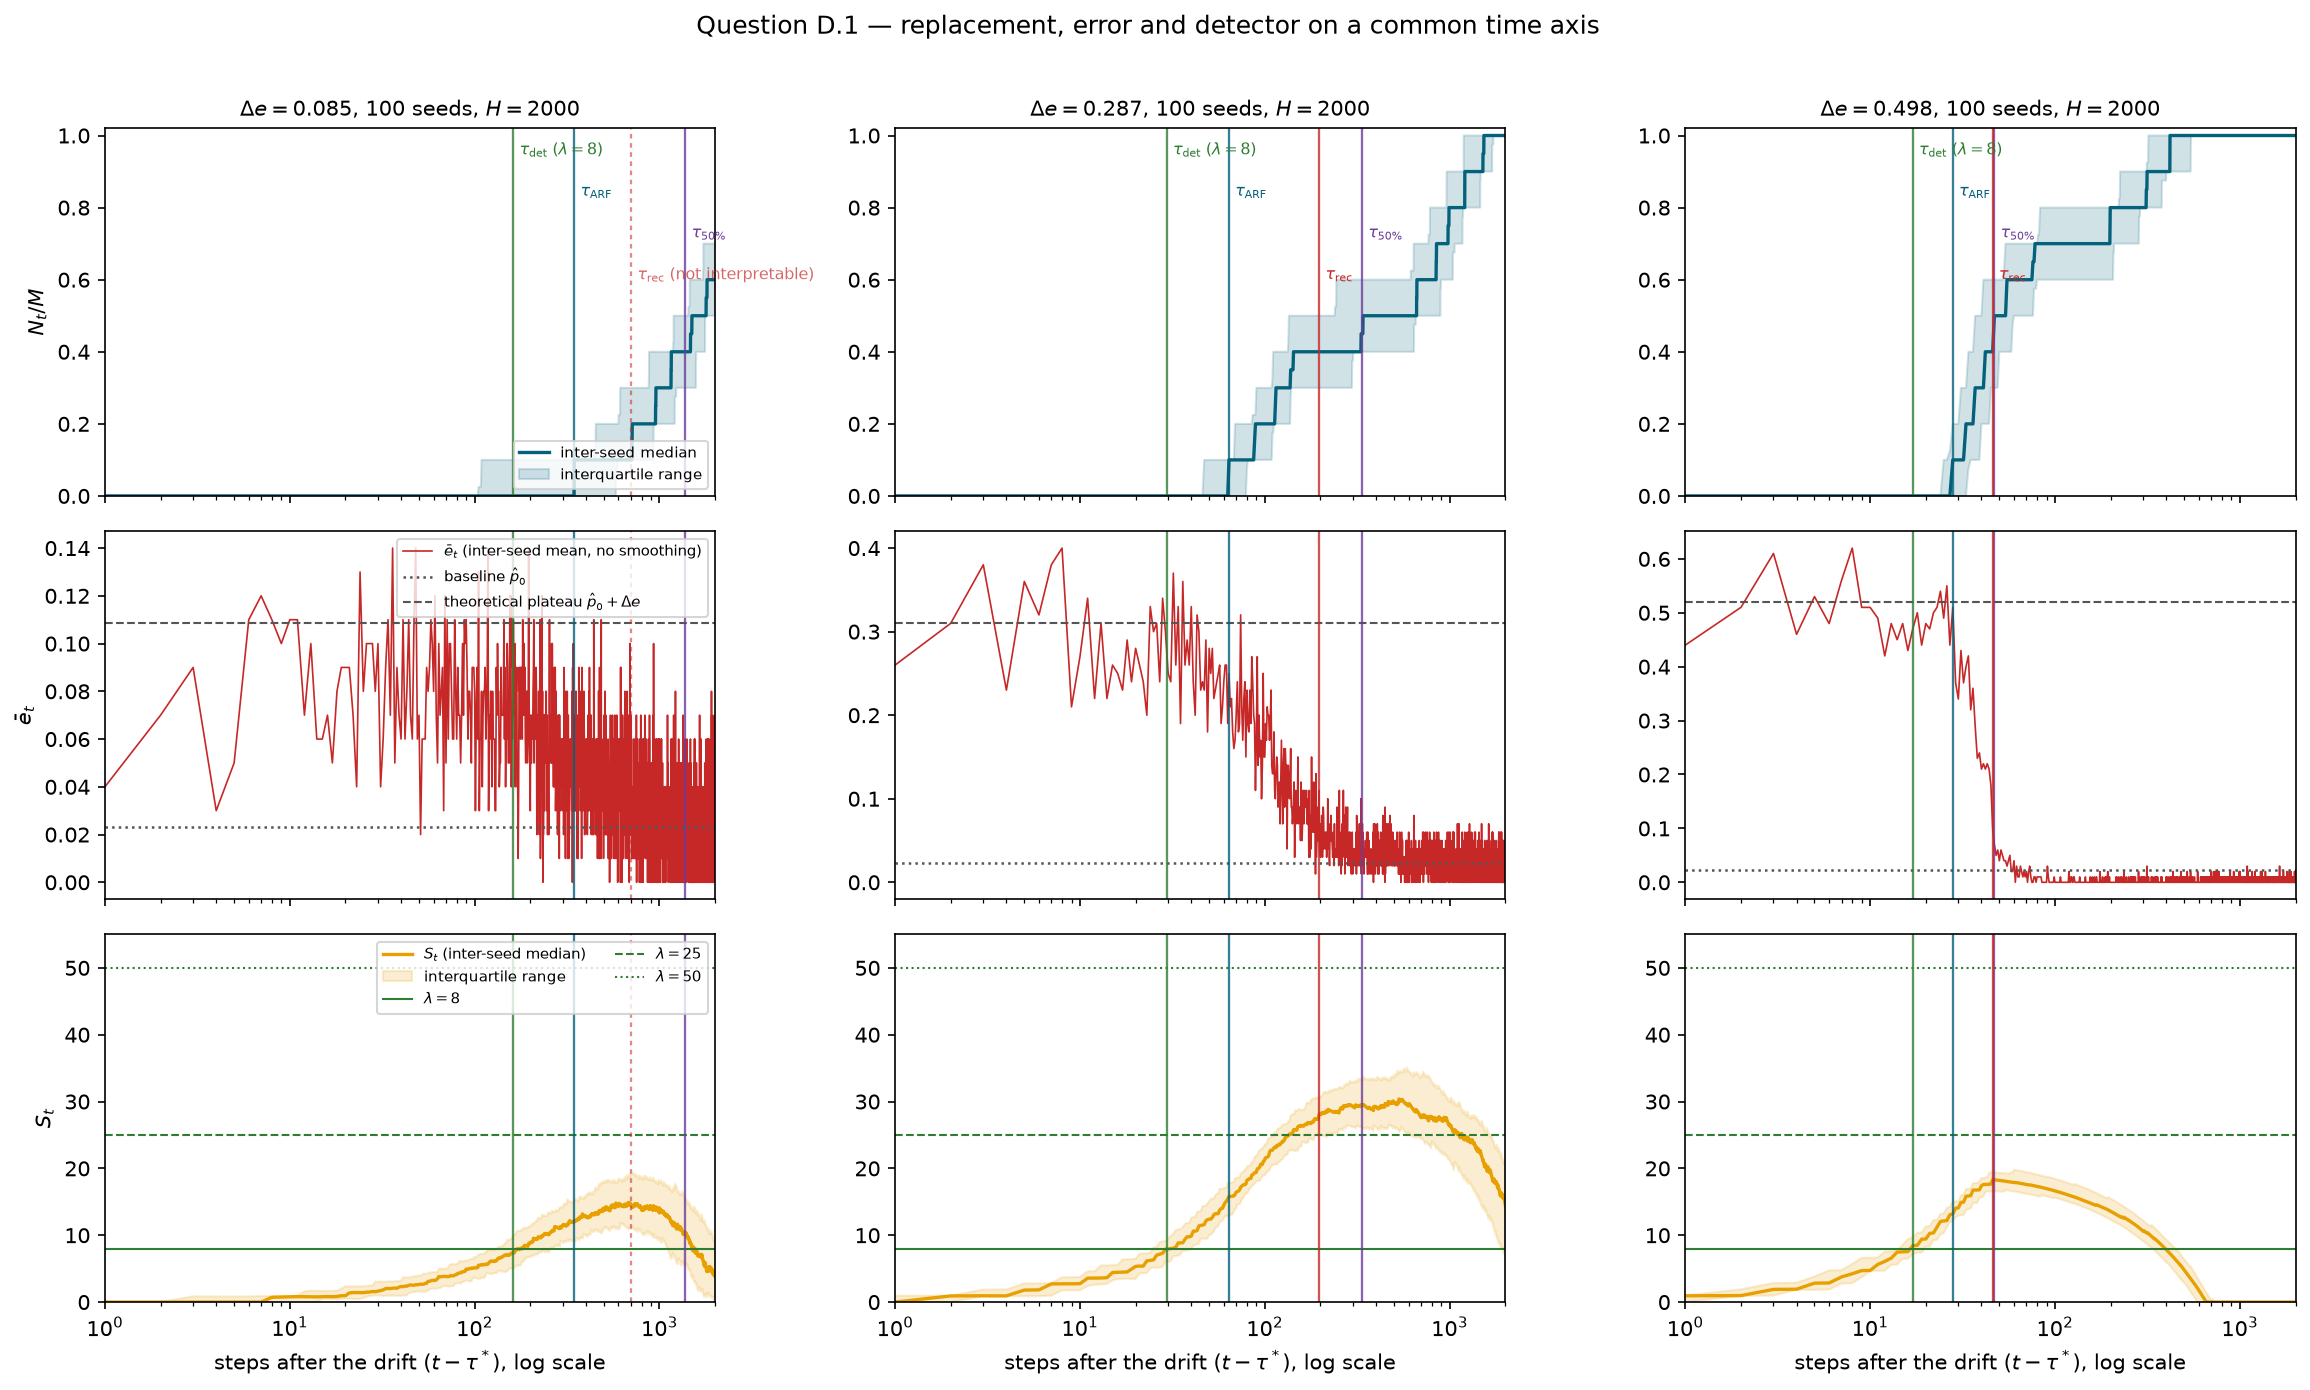
\includegraphics[width=\textwidth]{resultats_R2/resultats/figures/Fig_QD_trajectoires_full.png}
  \caption{$N_t/M$ (inter-seed median and IQR), global error $\bar e_t$, and detector state
  $S_t$ on a common time axis, at three amplitudes, with the four markers. Logarithmic
  axis: the instants span two orders of magnitude, and on a linear axis the markers of the
  right-hand column collapse into the first pixels. $\tau_{\mathrm{rec}}$ is dashed where
  the test lacks the power to resolve it.}
  \label{fig:joint}
\end{figure}

$e_t$ is binary and the only averaging is the inter-seed mean, step by step. No sliding
filter is used: one of length $L$ shifts the curve by half its support and destroys the
synchronisation with $\tau^*$, and at the top of the grid the median $\tau_{\mathrm{ARF}}$
is $28$ steps, so a $50$-step filter would displace it by nearly the quantity measured.

$\tau_{\mathrm{det}}$ is drawn at $\lambda = 8$, the only threshold whose censoring stays
in the minority ($4.70\%$, against $61.10\%$ at $\lambda = 25$, $99.95\%$ at
$\lambda = 50$); elsewhere a median would rest on a minority of runs and none is published.
$\tau_{\mathrm{rec}}$ is the return of the mean error below $\hat p_0 + \rho\,\Delta e$,
$\rho = 0.25$, held $20$ consecutive steps, written $\tau_{\mathrm{err}}(\rho)$ in Q~C.1.
The persistence does real work: without it two amplitudes cross at the first post-drift
step and two more at step $101$, well before the median $\tau_{\mathrm{ARF}}$, without the
crossing being sustained.

Replacement itself spans the grid. Median $N_t/M$ runs from $0.00$ to $0.70$ at $t=100$
(IQR $0.00$ to $0.30$), $0.10$ to $0.90$ at $t=400$, and $0.60$ to $1.00$ at the horizon,
where the share of fully renewed forests goes from $2\%$ to $94\%$.

\section{Baseline, on Both Windows}

$\hat p_0$ governs $\tau_{\mathrm{det}}$, $A(H)$ and $S_{\max}(H)$, hence every censoring
rate of Q~D.4, so both windows required by the protocol are reported. The $3\,000$
pre-drift steps recorded per run make this offline; as a control, the baseline recomputed
at $3\,000$ steps reproduces the campaign value with a deviation of exactly $0$.

\begin{table}[htbp]
  \centering
  \begin{tabular}{lcccc}
    \toprule
    Window & $\hat p_0$ (median) & \multicolumn{3}{c}{mean censoring of $\tau_{\mathrm{det}}$} \\
    \cmidrule(lr){3-5}
     & & $\lambda = 8$ & $\lambda = 25$ & $\lambda = 50$ \\
    \midrule
    $1\,000$ steps & $0.022000$ & $0.0405$ & $0.6045$ & $0.9990$ \\
    $3\,000$ steps & $0.023000$ & $0.0470$ & $0.6110$ & $0.9995$ \\
    \bottomrule
  \end{tabular}
  \caption{Maximum per-run difference between the two baselines: $0.009333$. The window
  shifts censoring by under one point and changes no verdict, though the direction is
  systematic: a longer window raises the baseline, so less evidence accumulates.}
  \label{tab:socle}
\end{table}

The theoretical baseline is exactly $0$: the pre-drift target
$y = \mathbf{1}\{x_0 + x_1 > 0\}$ is deterministic, with no label noise and zero Bayes
error. The measured $0.023$ is therefore entirely approximation error from axis-parallel
splits fitting an oblique boundary, so the detector monitors departures from a reference
level belonging to the classifier rather than to the problem.

\section{What Is Acquired at $\tau_{\mathrm{ARF}}$}

$R$ is the fraction of adaptation already acquired at $\tau_{\mathrm{ARF}}$, $G$ the
fraction of evidence already accumulated; $G$ is computed run by run, $R$ per amplitude on
the mean curve, $\tau_{\mathrm{ARF}}$ as the inter-seed median (Fig.~\ref{fig:rg}).

\begin{figure}[htbp]
  \centering
  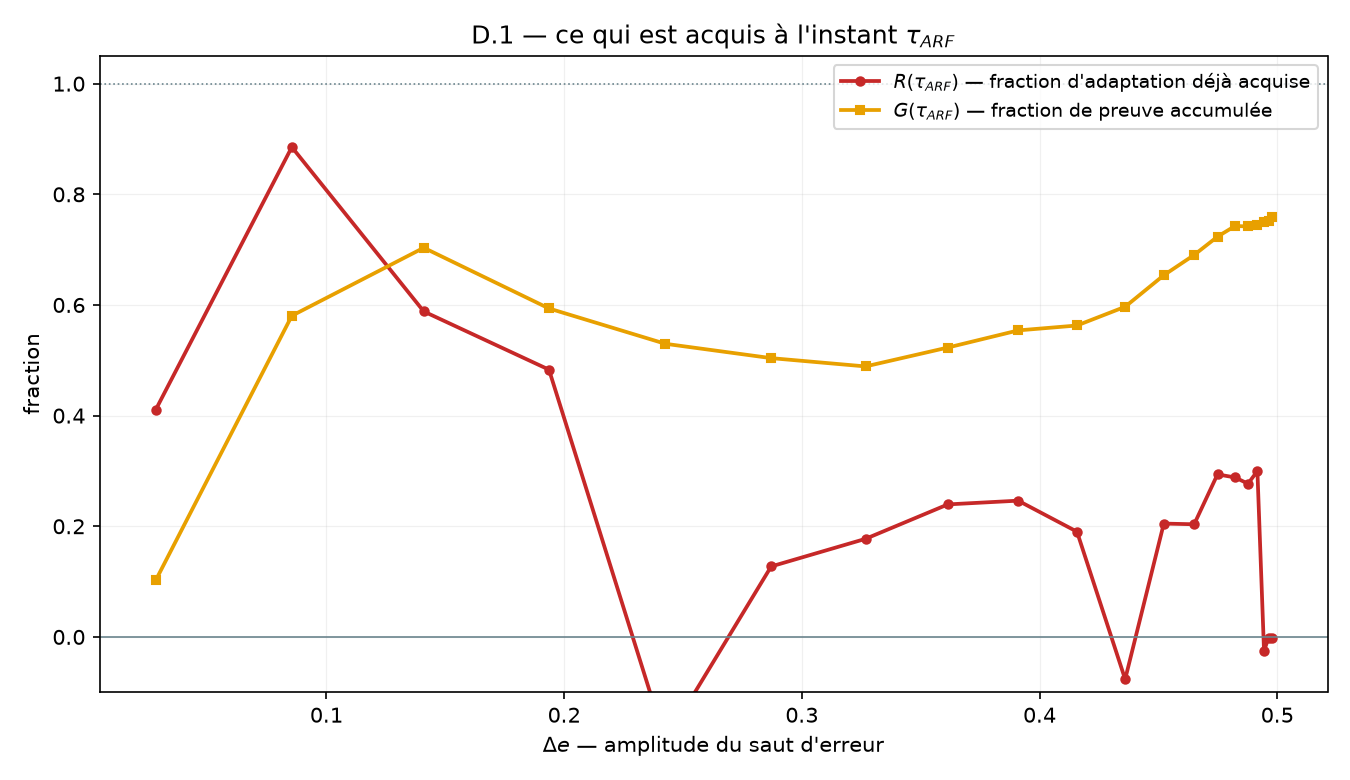
\includegraphics[width=0.72\textwidth]{resultats_R2/resultats/figures/Fig_QD_R_et_G_full.png}
  \caption{$R$ and $G$ against $\Delta e$. Neither is monotone; $R$ is negative at five
  amplitudes.}
  \label{fig:rg}
\end{figure}

$G$ ranges from $0.4889$ to $0.7594$ over the 18 amplitudes of the decision domain: half to
three quarters of the evidence is already available when the first tree is replaced. On the
full grid it falls to $0.1023$, and that restriction is published with the figure.

$R$ supports no single sentence. It runs from $-0.1882$ to $+0.8853$ on the grid, from
$-0.1882$ to $+0.5883$ on the decision domain, and is not monotone: at $\Delta e = 0.085$
it reaches $0.885$, so nearly all the adaptation is acquired when the first tree is
replaced, the opposite of what one would expect, and $0.588$ at $\Delta e = 0.141$. The
reading ``early in the adaptation, late in the race'' is not supported and is not used.
What holds is narrower: at $\tau_{\mathrm{ARF}}$ between $49\%$ and $76\%$ of the evidence
is accumulated, while the adaptation acquired varies from negative to $89\%$ with no
monotone dependence on amplitude.

$R$ is negative at $\Delta e = 0.243$, $0.436$, $0.494$, $0.496$, $0.498$, reaching
$-0.1882$. The plateau window is bounded by $\tau_{\mathrm{ARF}}/2$ to keep it from
overlapping the adaptation it measures, and the bound is active there ($43$, $17$, $14$,
$14$, $14$ steps), yet the symptom persists. A negative $R$ means the mean error at
$\tau_{\mathrm{ARF}}$ sits \emph{above} the plateau estimated just after the drift: the
error is still rising when the first tree is replaced. Calling this a repaired estimation
artefact would be false.

The plateau also never reaches $\hat p_0 + \Delta e$: the control fails on $20$ amplitudes
out of $20$, deviation between $-0.0271$ and $-0.0080$, always negative. Both mechanisms
point at the baseline. On the drift-free arm (100 runs, no change point) the forest still
performs a median of $14$ replacements and renews $9$ of its $10$ trees, for a mean error
of $0.0226$, so $\hat p_0$ is partly a product of the replacement mechanism. A comparison
against a forest that never replaces anything gave $0.0125$, but that comes from an
exploratory measurement of 12 executions (\texttt{JOURNAL.md} \S~2\,b) whose output was not
persisted and is quoted as an order of magnitude. Separately, at large amplitudes the
post-drift task is easier than the original one, so the error does not settle at
$\hat p_0 + \Delta e$ at all.

\section{The Race, Read from This Campaign}

At $\lambda = 8$, $\tau_{\mathrm{det}} < \tau_{\mathrm{ARF}}$ in $95.44\%$ of the $1\,906$
uncensored runs ($90.95\%$ of all $2\,000$ with censored runs imputed as losses); at
$\lambda = 25$, $6.56\%$; at $\lambda = 50$, $0\%$ on the single uncensored run. That
average needs a qualification: the rate is not stationary in $\Delta e$. At $\lambda = 8$
it is $0\%$ at $\Delta e = 0.028$, where $90\%$ of runs never alarm, $62\%$ at
$\Delta e = 0.085$, and $88\%$ to $99\%$ above. The $95.44\%$ is dominated by the 18 easy
amplitudes out of 20. The blind spot is a property of the pair $(\lambda, \Delta e)$ rather
than of $\lambda$ alone: even at the most sensitive threshold tested it is fully present at
the bottom of the grid.

\section{Not Addressed}

The official statement asks for the correlation of $\tau_{\mathrm{ARF}}$ with the residual
error and with the effective time of return to normal. The second is not computed as a
per-run correlation: $\tau_{\mathrm{err}}(\rho)$ is defined only on the seed-averaged
curve, one value per amplitude, since a single binary run is far too noisy for a threshold
crossing to signal recovery, whereas the correlations of Q~D are per run. The two are not
commensurable, and it appears only as the $\tau_{\mathrm{rec}}$ marker of
Fig.~\ref{fig:joint}. ``Return of the error to an acceptable level'' also fails as a
criterion: at $\Delta e = 0.498$ the threshold is crossed at step $46$, with or without
persistence, because the problem has become easier and the error falls below the pre-drift
baseline. Finally, the campaign exists at $M = 10$ only, so nothing in Q~D holds as a
function of forest size.

\end{document}
